
%Etat de l'art ________________________________________________________________________________________
\chapter {\'Etat de l'art}

L'information num\'erique et l'illustration sont des sujets vastes et pluridisciplinaires. Dans ce pr\'esent document, nous nous concentrerons sur ces concepts selon les aspects pertinents pour le projet. \par
\noindent L'\'etat de l'art de ce projet de sortie vise donc, d'une part, \`a pr\'esenter les moyens possibles de g\'erer et de distribuer des fichiers. D'autre part, il s'agira de pr\'esenter les principales tendances dans l'utilisation des illustrations. Nous chercherons \`a comprendre comment les informations num\'eriques sont stock\'ees, trait\'ees et transmises, ainsi que comment les illustrations sont utilis\'ees. Il sera \'egalement question de mettre en \'evidence  l'apport des illustrations en tant que vecteurs de communication, et d'explorer les cas o\`u elles sont utilis\'ees \`a des fins de communication.





\section{Concepts cl\'es}
%------------------------------------------------------------------L'information numerique--------------------------------------------------------------
Avant d'aller plus loin, commen\c{c}ons par pr\'esenter les deux concepts cl\'es autour desquels gravite ce projet.

\subsection{Information num\'erique}
\noindent Pour ce travail, nous d\'efinissons une information comme \lq\textit{Un \'el\'ement de connaissance qui peut \^etre enregistr\'e sur un support}\rq.\par
\noindent Une connaissance, en soi, \'etant immat\'erielle; g\'erer des informations revient donc le plus souvent \`a s'occuper de leur support. Dans le pass\'e, avec les supports physiques (bandes magn\'etiques, disques, livres, etc.), la gestion des informations n\'ecessitait \'enorm\'ement de ressources, tant humaines que financi\`eres. Aujourd'hui gr\^ace \`a l'essor de l'informatique, et surtout gr\^ace \`a Internet, nous utilisons des informations dont le support est un fichier num\'erique. Le support de l'information n'\'etant plus physique mais num\'erique, offre les avantages suivants:\\

\begin{itemize}
	\item[-] Un grand nombre de fichiers peuvent \^etre stock\'es sur un tr\`es petit composant mat\'eriel,\footnote{Un support de stockage. Ce concept sera mieux d\'etaill\'e par la suite} r\'eduisant ainsi l'encombrement physique des informations.
	\item[-] L'information peut \^etre g\'er\'ee via des outils informatiques.
	\item[-] L'information peut \^etre transmise via internet.\\
\end{itemize}

\vspace{0.5cm}

L'information num\'erique a apport\'e des avantages significatifs \`a la communication. En voici quelques uns:\\
\begin{itemize}
	\item[-] Le stockage co\^ute beaucoup moins cher
	\item[-] Les donn\'ees sont mieux prot\'eg\'ees contre la d\'et\'erioration physique
	\item[-] L'information occupe beaucoup moins d'espace physique
	\item[-] L'acc\`es devient plus rapide, n\'ecessite moins de ressources et demande tr\`es peu d'efforts
	\item[-] La transmission devient plus rapide, requiert moins de ressources et demande tr\`es peu d'efforts
	\item[-] La port\'ee de transmission est consid\'erablement augment\'ee, permettant de transf\'erer des informations d'un continent \`a un autre en une fraction de seconde.
\end{itemize}

\vspace{1cm}

\noindent Le num\'erique a tellement r\'evolutionn\'e le traitement de l'information, qu'il commence \`a s'int\'egrer dans tous les domaines de la vie quotidienne: l'\'education, la sant\'e, la m\'edecine, le commerce, le travail, etc.  En 2020, le march\'e mondial de l'apprentissage en ligne \'etait \'estim\'e \`a plus de 190 milliards de dollars US\cite{apprentissageEnLigne2020},  le march\'e mondial de la t\'el\'em\'edecine est pass\'e de 30.5 milliards de dollars US en 2019 \`a environ 41,2 milliards de dollars US en 2021\cite{marcheDeLaTelemedecine}, le march\'e mondial de la sant\'e num\'erique \'etait \'evalu\'e \`a plus de 330 milliards de dollars am\'ericains en 2022 \cite{DonneesSanteElectronique}. \`A titre de comparaison, le march\'e mondial EPC\footnote{Comprend les activit\'es d'ing\'enierie, d'approvisionnement et de construction pour les infrastructures p\'etroli\`eres et gazi\`ere} du p\'etrole et du gaz \'etait de 436 milliards de dollars US en 2023\cite{MarcheMondialPetrole}.

%-----------Illustration---------------------------------------------------------------------------------------------------------------
\subsection{Illustration}
Suivant le contexte, le terme illustration peut prendre plusieurs sens. Mais dans le cadre de notre travail, illustrer quelque chose, c'est lui associer une r\'ealisation particuli\`ere plus simple \`a comprendre que le cas g\'en\'eral. Ainsi, illustrer une information, repr\'esente la pr\'esentation d'une situation dans laquelle cette information est mise en \'evidence. Pour \^etre plus clair, illustrons d'ailleurs cela.\\
Disons que l'on veut faire passer cette information: \emph{"Il ne faut pas construire pr\`es des ravins ou autres cours d'eau"}. Une illustration de cette information pourrait \^etre un r\'ecit (sous forme de texte, audio ou vid\'eo) qui raconte l'histoire suivante:
\begin{quotation}
	\texttt{M. Dieudonn\'e et M. Pierre-Richard sont deux amis, voisins et p\`eres de famille. M. Pierre-Richard a construit sa maison trop pr\`es d'une rivi\`ere tandis que M. Dieudonn\'e a gard\'e une distance de s\'ecurit\'e. Un ouragan a touch\'e la r\'egion, la maison de M. Pierre-Richard a \'et\'e inond\'ee et il a d\^u se r\'efugier, lui et sa famille chez son ami qui n'avait pas ce probl\`eme.}
\end{quotation}

\noindent Ce pourrait aussi \^etre
\begin{quotation}
	\ttfamily Une image montrant deux maisons pendant un ouragan. L'une, construite au mauvais endroit a \'et\'e inond\'ee tandis que l'autre construite au bon endroit n'a pas \'et\'e innond\'ee.( Voir figure~\ref{FigKonstuiBoRivye}) \normalfont

\end{quotation}

\noindent Ou encore,

\begin{quotation}
		\ttfamily une sculpture repr\'esentant l'eau d'un ravin qui ravage tout ce qui est sur ses bords, inonde les maisons, d\'etruit les plantations, emporte les arbres et les animaux qu'elle trouve, tandis qu'\`a partir d'une certaine distance, elle ne peut atteindre ni les gens ni leurs biens.\normalfont
\end{quotation}

	\paragraph{} Dans la suite de ce document nous utiliserons le terme illustration soit pour d\'esigner la r\'ealisation particuli\`ere qu'on associe \`a une information, soit pour d\'esigner le fichier num\'erique qui contient cette r\'ealisation particuli\`ere.\par

\noindent L'illustration, telle que d\'efinie ci dessus,  a toujours fait parti du folklore ha\"itien. On peut le retrouver sous forme de dictons\footnote{comme dans: \emph{\lq Kisa Frize te f\`e pou Koukou, pou Koukou ta f\`e pitit li, li rele l Frizelya?"}}, ou dans la musique\footnote{\textit{Sou chimen p\`edi tan\rq} de Carole Demesmin ; \textit{\lq Tinonm\rq} de B\'elony Murat di B\'elo}, le th\'eatre \footnote{\textit{Lavi nan bouk} de Jean-Claude Joseph dit Papa Py\`e}, etc. Elles sont aussi utilis\'ees pour sensibiliser la population ou diffuser des messages d'alerte. A titre d'exemple, on peut citer les vid\'eos illustr\'ees que passaient les cha\^ines de t\'el\'evision locales (Notamment la TNH\footnote{T\'el\'evision Nationale d'Ha\"iti}) pour sensibiliser les gens \`a ne pas jeter des d\'echets dans les ravins lorsqu'il pleut\cite{TiJowelOuJetreFatraADeja}, \`a ne pas uriner sur la place publique\cite{DegajePaPeche}, etc. ou les illustrations graphiques (voir figure~\ref{LaveMenNouPouNouPaTrapeKowona}) qui, pendant la pand\'emie Covid-19,  \'etaient affich\'ees dans les rues pour encourager le lavage des mains \`a la population afin de lutter efficacement contre le virus.


\begin{figure}[h]
	\begin{minipage}{0.5\textwidth}
		\centering
		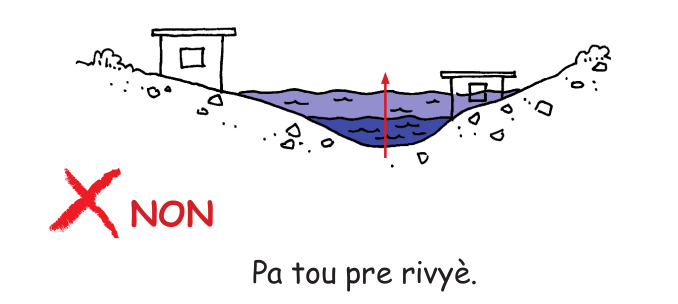
\includegraphics[width=\textwidth]{Pictures/KonstuiBoLarivye.png}
		\caption{Exemple d'illustration}
		\label{FigKonstuiBoRivye}
	\end{minipage}
	\begin{minipage}{0.5\textwidth}
		\centering
		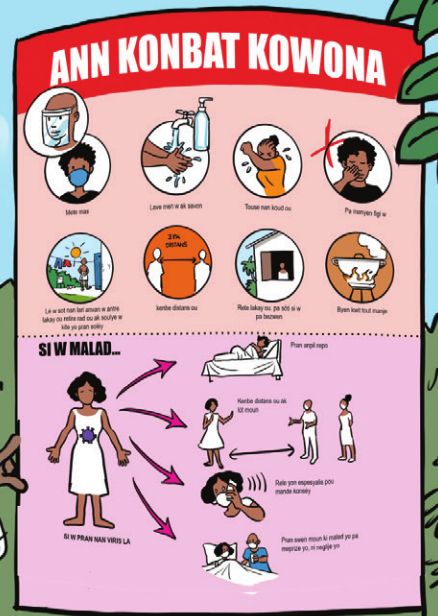
\includegraphics[height=0.3\textheight]{Pictures/AfichKontKowona.png}
		\caption{Affiche pour la sensibilisation contre le Covid-19}
		\label{LaveMenNouPouNouPaTrapeKowona}
	\end{minipage}
\end{figure}








\section{Avanc\'ees dans le domaine des syst\`emes d'information (SI)}
Suivant la probl\'ematique, nous devons construire un syst\`eme capable de rendre des fichiers num\'eriques accessibles.
% Le moyen le plus utilis\'e pour cela est d'entreposer les ressources \`a distribuer, et fournir l'acc\`es \`a cet entrep\^ot.
Un tel syst\`eme est appel\'e syst\`eme d'information.%\cite{DefinitionDeSI}\\


\noindent Un syst\`eme d'information permet de collecter des documents, de les stocker , de les traiter puis de les distribuer \`a la demande d'une personne tierce. Dans le cas o\`u les donn\'ees \`a manipuler sont des informations num\'eriques(fichiers ou donn\'ees), chacune des quatre fonctions du syst\`eme (collecter, stocker, traiter et communiquer) est assur\'ee par un ensemble de mat\'eriels informatiques, d'outils logiciels, de technologies et de proc\'edures. Le syst\`eme en soi sera r\'ealis\'e en connectant les diff\'erentes parties de mani\`ere \`a ce que l'ensemble puisse fournir une interface utilisateur ainsi que les services requis.

\subsection{Stockage de fichier dans le SI}
Le stockage d'information se r\'ef\`ere \`a la conservation de l'information. Cette t\^ache doit \^etre effectu\'ee de mani\`ere efficace, efficiente et s\'ecuris\'ee. En ce qui concerne le stockage d'information num\'erique, les avanc\'ees touchent notamment les supports sur lesquels les informations sont stock\'ees (les supports de stockage), les m\'ethodes permettant aux syst\`emes informatiques d'acc\'eder \`a l'espace de stockage (les solutions et technologies de stockage) et la forme sous laquelle les informations seront tra\^it\'ees.



\subsubsection{Supports de stockage}
Un p\'eriph\'erique de stockage est un composant \'electronique sur lequel on enregistre des donn\'ees num\'eriques. Il en existe plusieurs types (Carte SD, USB Flash Drive, Disque dur, etc.).\\
Chaque p\'eriph\'erique est caract\'eris\'e par sa volatilit\'e, sa capacit\'e de stockage, la vitesse \`a laquelle il peut lire ou \'ecrire des donn\'ees , la quantit\'e de donn\'ees qu'il peut transmettre par unit\'e de temps et la dur\'ee pendant laquelle il peut conserver des donn\'ees sans les alt\'erer.\\

\begin{itemize}
	\item[-] \textbf{La volatilit\'e} d\'ecrit le comportement du p\'eriph\'erique lorsqu'il est mis hors tension. Un p\'eriph\'erique est dit \emph{volatil} s'il perd les donn\'ees d\`es qu'il est mis hors tension, et \emph{non-volatil} si, dans le m\^eme cas, il les conserve pour un certain temps.\\
	\item[-] \textbf{La capacit\'e} d'un p\'eriph\'erique est la quantit\'e maximale de donn\'ees qu'il peut conserver. Elle est exprim\'ee en bytes (ou octet).
\end{itemize}



\paragraph{} \'Etant donn\'e que notre projet vise \`a stocker des informations de fa\c{c}on p\'erenne pour les distribuer ensuite. Les donn\'ees doivent n\'ecessairement \^etre stock\'ees sur des p\'eriph\'eriques non-volatils, de grande capacit\'e et avec une vitesse d'acc\`es ad\'equate. Ils doivent \'egalement offrir une vitesse de lecture raisonnable afin de limiter le temps de r\'eponse des requ\^etes effectu\'ees sur le syst\`eme et d'augmenter le nombre maximal d'acc\`es simultann\'es aux donn\'ees. \\
Parmi les p\'eriph\'eriques de stockage disponibles sur le march\'e, ceux qui r\'epondent \`a ces crit\`eres (non-volatil et de grande capacit\'e) sont d\'enomm\'es \emph{p\'eriph\'erique de stockage secondaire}\cite{stockagesSecondaire}. Les principaux sont les suivants.\\

\begin{itemize}
	\item[-] \textbf{P\'eriph\'erique de stockage magn\'etique}
	Le stockage magn\'etique utilise des bandes ou des disques recouverts d'un mince rev\^etement magn\'etique qui permet de conserver les donn\'ees sous forme de particules magn\'etique\cite{stockagesSecondaireMagnetique}. Le support le plus commun\'ement utilis\'e pour stocker des donn\'ees num\'eriques est  le disque dur(Hard disk Drive)\cite{stockagesSecondaireMagnetique}.\\

	\item[-] \textbf{P\'eriph\'erique de stockage SSD (Solid State Drive)\cite{stockagesSecondaire}}
	Le stockage SSD utilise des puces m\'emoires \'electroniques pour conserver les donn\'ees sous forme de charge \'electrique\cite{stockagesSecondaireElectrique}. Le p\'eriph\'erique SSD est tr\`es semblable au disque HDD. Les principales diff\'erences sont que: le SSD, utilise moins d'\'energie pour fonctionner, il est moins fragile, permet d'acc\'eder aux donn\'ees \`a une plus grande vitesse\cite{stockagesSecondaireElectrique}, et il est plus performant pour les acc\`es concurrentes en lecture ou en \'ecriture, bien qu'il ait une dur\'ee de vie moindre.\\

	\item[-] \textbf{RAID ( Redundant array of independent disks)\cite{MethodesEtTechnologies}\cite{MethodesEtTechnologies1}} \\
	Le RAID est une m\'ethode de stockage de donn\'ees qui consiste \`a utiliser plusieurs p\'eriph\'eriques de stockage ind\'ependants pour stocker les m\^emes donn\'ees. Avec cette m\'ethode, les donn\'ees sont organis\'ees de mani\`ere \`a ce que, si l'un des p\'eriph\'eriques tombe en panne, les autres suffisent pour reconstituer l'ensemble des donn\'ees que contenait le syst\`eme avant la panne. \par
	\noindent Le RAID permet de construire un syst\`eme tol\'erant aux pannes. Cette m\'ethode augmente la performance et la fiabilit\'e du syst\`eme de stockage.\\
\end{itemize}



\subsubsection{Solutions et technologies de stockage}
Au fil du temps, le fait de conserver les donn\'ees, en soi, s'est av\'er\'e insuffisant pour un stockage efficace et efficient. Il est devenu tout aussi important d'assurer la disponibilit\'e des donn\'ees, d'y bloquer l'acc\`es non-authoris\'e, de prot\'eger les syst\`emes contre les pannes et d'autres al\'eas. Ainsi de nombreuses m\'ethodes et technologies ont \'et\'e d\'evelopp\'ees pour aider \`a la conception, la gestion et la maintenance des syst\`emes de stockage. Chaque m\'ethode ou technologie est caract\'eris\'ee par un ensemble d'avantages et de contraintes, et ce sont ces caract\'eristiques qui serviront de base pour choisir quels moyens de stockage \`a adopter.\\

\begin{itemize}
	\item[-] \textbf{P\'eriph\'erique attach\'e\cite{MethodesEtTechnologies}\cite{MethodesEtTechnologies1}}\\
	C'est la m\'ethode utilis\'ee par d\'efaut pour fournir de l'espace de stockage aux ordinateurs. Elle consiste \`a attacher le p\'eriph\'erique de stockage directement \`a un ordinateur (PC, Desktop, Serveur). Cette m\'ethode permet d'allouer toute l'espace de stockage d'un p\'eriph\'erique \`a un seul ordinateur. Elle est la moins co\^uteuse, et offre une bonne performance. Mais elle est peu tol\'erante aux pannes. \\

	\item[-] \textbf{NAS (Network Attached Storage)}\\
	Cette m\'ethode consiste \`a d\'eployer un syst\`eme de stockage sous forme de serveur sur un r\'eseau. Ce syst\`eme fournit le stockage aux clients du r\'eseau comme un service. Les clients acc\`edent \`a ce syst\`eme de stockage via son addresse IP. \\

	\item[-] \textbf{SAN (Storage Area Network)\cite{MethodesEtTechnologies}\cite{MethodesEtTechnologies1}} \\
	Cette m\'ethode consiste \`a regrouper plusieurs p\'eriph\'eriques de stockage, de m\^eme type ou de types diff\'erents, en un seul grand syst\`eme de stockage qui servira d'espace de stockage \`a un ensemble de ressources informatiques. Cette solution offre une tr\`es grande performance et une haute disponibilit\'e des donn\'ees mais, elle est \'egalement tr\`es co\^uteuse.\\

	\item[-] \textbf{Stockage en nuage (Storage As A Service)\cite{MethodesEtTechnologies}\cite{MethodesEtTechnologies1}} \\
	Il s'agit de louer de l'espace de stockage aupr\`es d'un fournisseur. Le client peut acc\'eder \`a ses donn\'ees via Internet. Cette m\'ethode permet de se passer des co\^uts de d\'eploiement d'un syst\`eme de stockage local et de g\'erer les grandes fluctuations dans l'espace de stockage utilis\'e, en ne payant que pour ce qui est effectivement consomm\'e.\\

\end{itemize}

\subsubsection{Logiciels pour le stockage\cite{systemDeFichiers}\cite{UitiliteDesBaseDeDonnees}}
	Les informations num\'eriques peuvent \^etre stock\'ees soit sous forme de donn\'ees, soit sous forme de fichiers. \textit{Une donn\'ee est un fait observ\'e mais pas encore interpr\'et\'e}. Une fois interpr\'et\'ee, la donn\'ee devient une information. \textit{Un fichier est une collection structur\'ee de donn\'ees concernant un m\^eme sujet, r\'eunie sous un m\^eme nom}.



	\paragraph{} \textbf{Syst\`eme de fichiers}\\
	Un syst\`eme de fichiers fournit un environnement dans lequel des fichiers peuvent \^etre tra\^it\'es. Il est compos\'e d'un ensemble de fichiers et d'une structure de dossiers qui organise ces fichiers et fournit des informations sur chacun d'eux. Les ordinateurs sont g\'en\'eralement \'equip\'e d'un syst\`eme de fichiers built-in et d'un logiciel permettant de le g\'erer. Toutefois il est possible d'en programmer d'autres si n\'ecessaire.\\
	Cette m\'ethode est tr\`es efficace pour tra\^iter des informations sous forme de fichiers, mais elle s'est av\'er\'ee inefficace et non-adapt\'e \`a l'utilisation et la gestion de donn\'ees\cite{systemDeFichiers}. D'o\`u l'int\'er\^et des bases de donn\'ees\cite{DefinitionDeFichier2}.




	\paragraph{}\textbf{Base de donn\'ees}\\
	Une base de donn\'ees est une structure informatique qui sert \`a contenir une collection de donn\'ees et permet de les exploiter\cite{BaseDeDonnees}.
	Pour cr\'eer et/ou utiliser une base de donn\'ees, il est n\'ecessaire d'utiliser un Syst\`eme de Gestion de Base de Donn\'ees (SGBD). Il en existe plusieurs, tels que: Microsoft Access, MySQL, Oracle Database, OrientDB ou CouchDB.




	\subsection{Collecte, traitement et distribution des fichiers}
	En r\'eponse \`a la probl\'ematique, notre syst\`eme doit \^etre capable de transmettre des fichiers vers un maximum de personnes. Puisqu'il s'agit de fichiers num\'eriques, chaque personne doit disposer d'un syst\`eme informatique (Laptop, Desktop, Smartphone, tablette, etc.). Pour qu'un syst\`eme informatique puisse communiquer avec un autre, il doit s'interfacer (se mettre en r\'eseau) avec les syst\`emes avec lesquels il souhaite \'echanger des informations . Nous devons donc mettre notre syst\`eme en r\'eseau. Puisque nous voulons communiquer avec un maximum de personnes, nous devons utiliser Internet, qui est le plus grand des r\'eseaux informatiques. \\
	Nous devons donc d\'evelopper un syst\`eme d'information num\'erique accessible via Internet. Un moyen de faire cela est de construire une application web\cite{ApplicationWeb} qui fournit le service de transfert de fichiers.\\

\paragraph{} Dans une application web, la collecte et le traitement de fichiers sont impl\'ement\'es comme des services. Ces fonctions sont r\'ealis\'es par les  proc\'edures d'une application serveur.\\
Les avanc\'es, en ce qui concerne la cr\'eation de services dans une application web concernent notamment le langage de programmation et les frameworks utilis\'es. (\cite{techstack})

\subsubsection{Technologies de d\'eveloppement}
%			Comme nous venons de le voir, le syst\`eme d'information doit \^etre impl\'ement\'e \`a travers
Une application web est un programme informatique accessible via un navigateur\cite{ApplicationWeb}. Le d\'eveloppement d'une application web requiert l'utilisation de langage de programmation et d'autres outils et technologies utilis\'es dans la programmation.\\

\begin{itemize}
	\item[-] Interface utilisateur (Front-End)\cite{frontendprogramming}\\
	Pour d\'evelopper l'interface utilisateur, on peut utiliser HTML, CSS et JavaScript, ou opter pour un framework bas\'e sur ces langages comme Angular, Vue ou React.
	\item[-] D\'eveloppement c\^ot\'e serveur (Back-End)\cite{backendprogramming}\\
	L'impl\'ementation des fonctions (collecte, traitement et distribution), requiert de coder les proc\'edures qui vont fournir les services n\'ecessaires et utiliser des requ\^etes pour communiquer avec la base de donn\'ees. Pour cela, il faut utiliser un langage de programmation tel que PHP, Python, Ruby, Java ou C\#. Il faudra ensuite choisir un framework bas\'e sur le langage s\'electionn\'e. Parmi les framework fr\'equemment utilis\'es, on peut citer: Express, Spring, Django, Laravel, Rails, et .NET.
	\item[-] Base de donn\'ees\\
	Pour construire une base de donn\'ees, nous devons d'abord choisir un syst\`eme de gestion de base de donn\'ees suivant les besoins de l'application. Il en existe beaucoup. Parmi les plus connus: MySQL, PostgreSQL, MongoDB, MariaDB, etc.\\
	Ensuite, il faut cr\'eer un mod\`ele de donn\'ees qui servira de base pour \'elaborer le sch\'ema des donn\'ees en utilisant le langage du SGBD choisi.


\end{itemize}






\section{L'illustration en Ha\"iti et dans le monde}
\label{SectionAvantageIllustrations}
L'illustration, telle que d\'efinie dans l'introduction, est omnipr\'esente dans la vie quotidienne. On la retrouve dans des r\'ecits oraux, des livres, les journaux, les magazines, les affiches, les bandes dessin\'ees, les jeux vid\'eo, les films d'animation, etc. \\
Suivant le format de document num\'erique utilis\'e, une illustration peut \^etre une image, un texte, un fichier audio ou un fichier vid\'eo.


\subsection{Importance de l'illustration}
Le fait d'utiliser des illustrations pr\'esente plusieurs avantages. Voici une liste non-exhaustive de leurs traits b\'en\'efiques qui pourraient \^etre exploit\'es dans notre syst\`eme.

\subsubsection{Expliquer simplement}
Les illustrations permettent d'expliquer facilement des concepts qui pourraient \^etre complexes et difficiles \`a comprendre \`a travers des expos\'es explicatifs classiques. Des illustrations sont utilis\'ees \`a cet effet dans des  livres, des articles, des sites Web, etc. La figure~\ref{CiscoReseau} montre un cas o\`u le concept de transfert de message est illustr\'e dans le livre `` CCNP and CCIE Enterprise Core `` de Cisco.


\begin{figure}[ht]
	\centering
	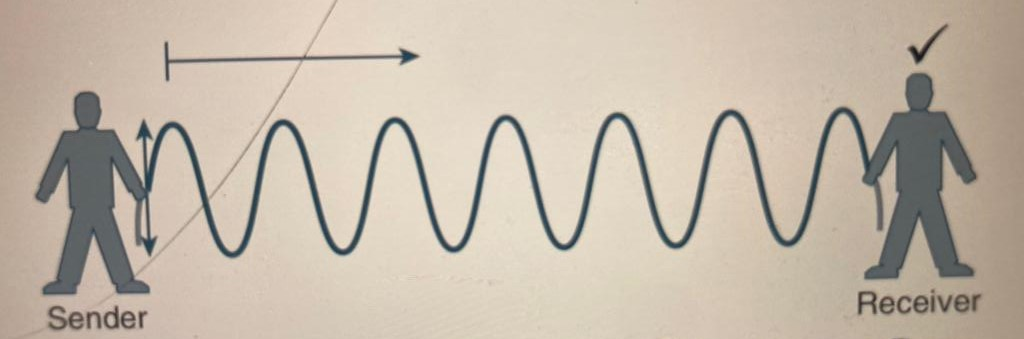
\includegraphics[width=0.75\linewidth]{Pictures/Sending Message.jpg}
	\caption{Illustration d'un transfert de message\cite{CiscoMessage}}
	\label{CiscoReseau}
\end{figure}


\subsubsection{Susciter l'engagement du spectateur}
Les illustrations peuvent rendre des contenus beaucoup plus engageant en cr\'eant un contexte dans lequel le spectateur peut s'identifier pleinement. Par exemple, elles sont utilis\'ees dans les livres pour enfants, pour les garder engag\'es dans la lecture et stimuler leur int\'er\^et pour la lecture comme dans ''The three questions'' by Jon J. Muth. De m\^eme, dans la vid\'eo illustr\'ee intitul\'ee ''Ey chof\`e, P\`otay ou prale?'' utilis\'ee par la T\'el\'evision Nationale d'Ha\"iti (TNH) pour sensibiliser la population \`a respecter les feux de signalisation sur les routes. Le contexte, notamment, la destination du personnage (Portail L\'eoganne), les camionnettes, les intervenants, le d\'ecor en g\'en\'eral, rappelle l'environnement ha\"itien et incite un ha\"itien qui regarde la vid\'eo \`a se sentir concern\'e par le contenu.\\


\subsubsection{Faciliter la m\'emorisation du contenu}
La m\'emorisation est le fait de conserver des informations pour pouvoir s'en rappeler apr\`es un certains temps. De nombreux facteurs  internes ou externes (attention, sant\'e, alimentation, hygi\`ene de vie, fr\'equence \`a laquelle nous acc\'edons \`a l'information, la valeur \'emotionnelle qu'on lui accorde ) peuvent affecter la m\'emorisation d'une information soit en la facilitant, soit en la rendant plus compliqu\'ee.  Les illustrations peuvent \^etre utilis\'ees pour faciliter la m\'emorisation :\\

\begin{itemize}
	\item[-] Dans une illustration, chaque \'el\'ement d'information est situ\'e dans un contexte bien d\'efini, de sorte qu'il puisse \^etre li\'e aux autres informations constituant l'illustration. \cite{ContextDependencyEffect}
	\item[-] Les illustrations graphiques et vid\'eos offrent une repr\'esentation visuelle directe, ce qui rend les informations plus faciles \`a retenir. \cite{ImageMemoire} \cite{ImageMemoireb}
	\item[-] Certaines illustrations repr\'esentent des r\'ecits narratifs dans lesquels l'information utile est introduite. Cette approche narrative rend le contenu plus facile \`a m\'emoriser.\cite{NarrationMemoire}
\end{itemize}
Par cons\'equent, L'utilisation d'illustrations augmente les chances que les personnes qui visionnent les documents se souviennent des informations re\c{c}ues.


\subsection{Utilisations faites des illustrations}


\subsubsection{Attirer l'attention}
Des illustrations tr\`es color\'ees sont utilis\'ees pour inciter les gens \`a pr\^eter attention au contenu. Elles sont souvent employ\'ees dans les livres pour enfant (Comme Le petit prince de \cite{LePetitPrince}) ou en marketing comme le montre l'affiche publicitaire de la figure~\ref{FigMaltaH}.



\begin{figure}[ht]
	\centering
	
\includegraphics[width=0.50\linewidth]{Pictures/MaltaH.jpg}
	\caption{Affiche publicitaire illustr\'ee visant \`a attirer l'attention}
	\label{FigMaltaH}
\end{figure}



\subsubsection{Rendre des informations plus accessibles}
Les illustrations sont utilis\'ees pour rendre des informations plus accessibles. Elles permettent de communiquer avec les personnes atteintes de c\'ecit\'e ou de troubles auditifs, pourvu qu'elles disposent de l'un ou l'autre de ces sens, l'ou\"ie et la vue. Elles ne requi\`erent pas beaucoup de temps pour transmettre le message, ce qui est avantageux pour ceux qui n'ont pas beaucoup de temps pour s'informer. Certaines illustrations utilisent une forme d'expression intuitive ne n\'ecessitant pas de connaissances sp\'ecifiques pour \^etre interpr\'et\'ees. Ainsi elles permettent de communiquer efficacement notamment avec les enfants, mais aussi avec les membres de la communaut\'e qui sont analphab\`etes (soit plus de 48\% de la population locale  en 2018\cite{AnalphabetismeHaiti}) ou qui pr\'esentent certains autres formes de limitation intellectuelle.

\subsubsection{Communiquer}
Les illustrations sont utilis\'ees pour communiquer des messages. Notamment pour faire face \`a une \'epid\'emie (Voir Figure~\ref{FigCovid}), une catastrophe naturelle (Voir Figure~\ref{ConsigneSeisme}) ou pour s'adresser aux enfants (Voir Figure~\ref{ConsigneToillette}), on en fait souvent usage. Elles sont aussi tr\`es utilis\'ees pour faire passer des avertissements (Voir Figure~\ref{Avertissement}).

	\begin{figure}[ht]
		\vspace{10pt}
		\centering
		\begin{minipage}{0.45\textwidth}
			\centering
			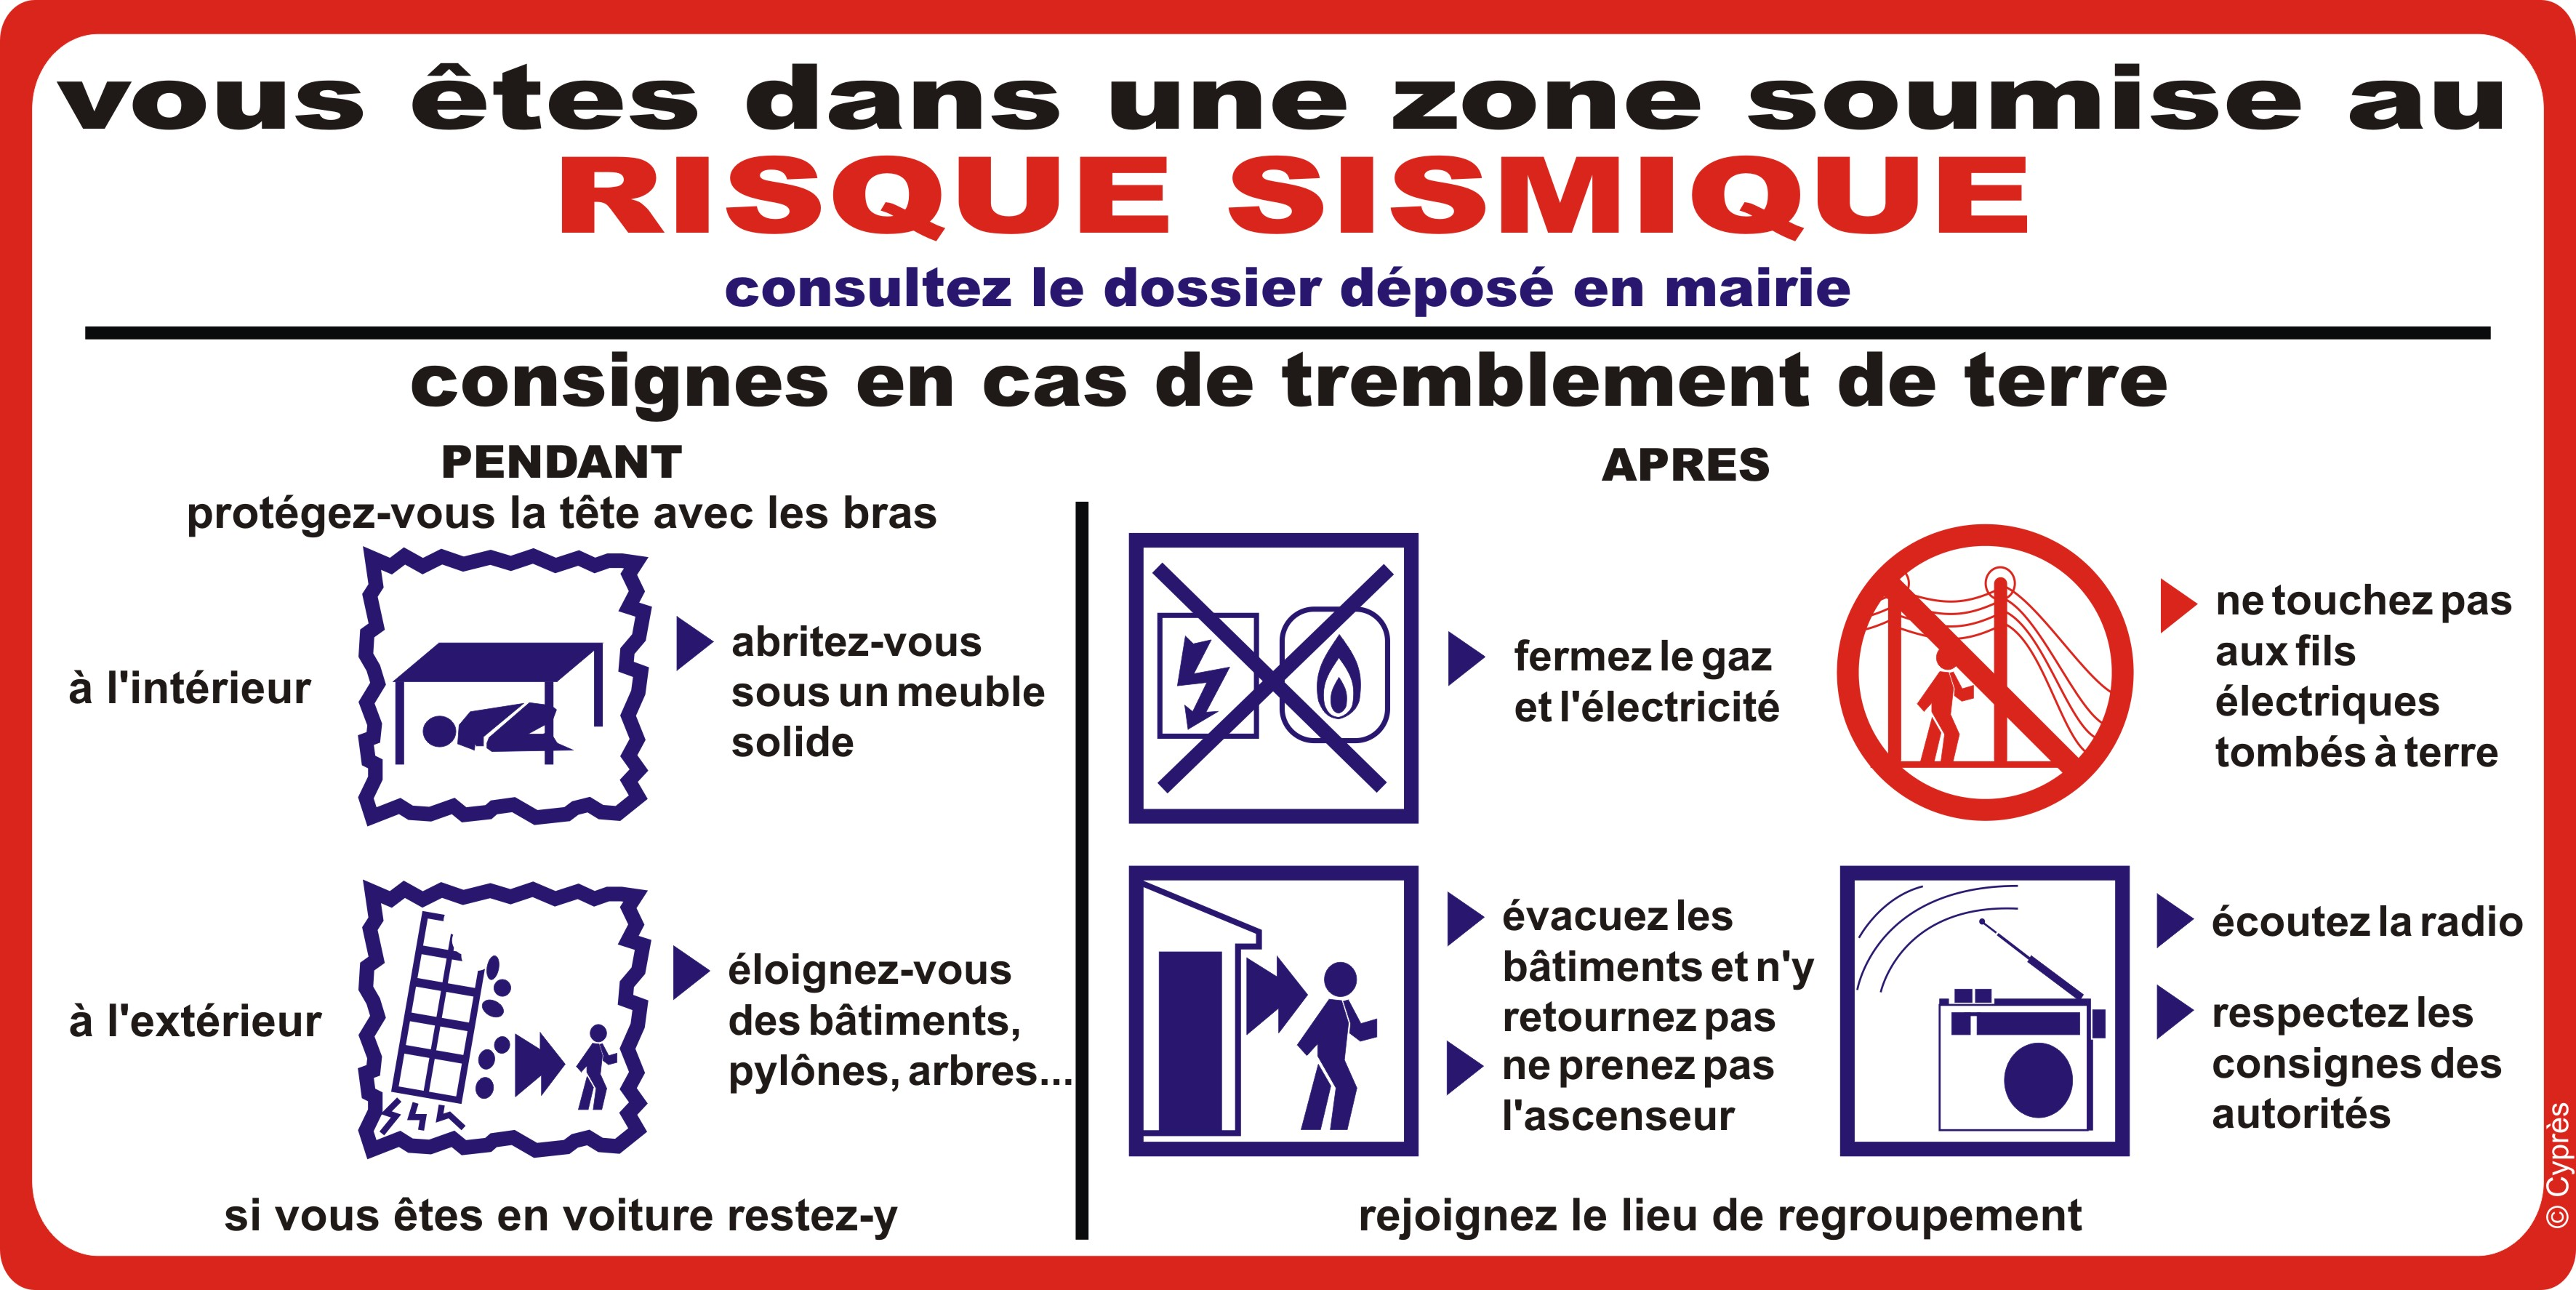
\includegraphics[width=5cm]{Pictures/RisqueSismique.jpg}
			\caption{Illustration des consignes pour se prot\'eger pendant et apr\`es un s\'e\"isme}
			\label{ConsigneSeisme}
		\end{minipage}
		\hspace{10pt}
		\begin{minipage}{0.45\textwidth}
			\centering
			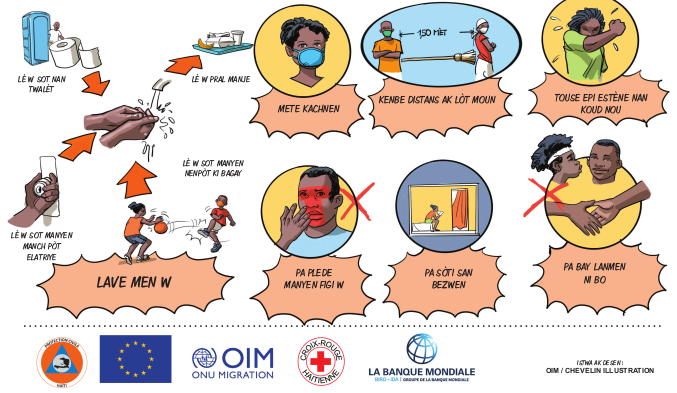
\includegraphics[width=5cm]{Pictures/FigCovid.png}
			\caption{Illustration des consignes pour se prot\'eger contre le Covid-19}
			\label{FigCovid}
		\end{minipage}

		\vspace{10pt}

		\begin{minipage}{0.45\textwidth}
			\centering
			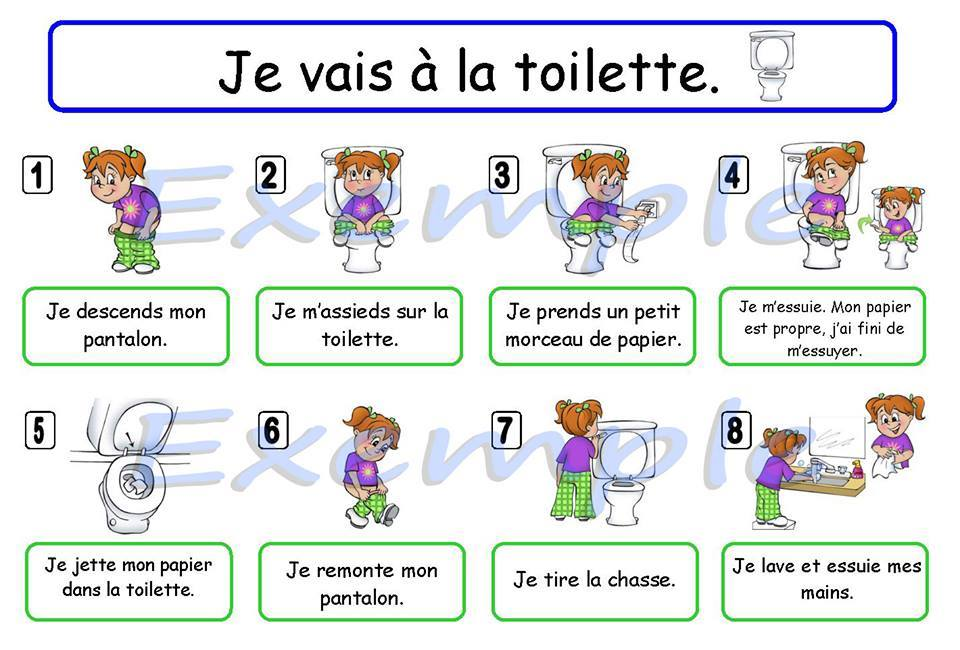
\includegraphics[width=5cm]{Pictures/SeServirDeLaToilettePourEnfant.jpg}
			\caption{Illustration enseignant aux enfants comment se servir des toilettes}
			\label{ConsigneToillette}
		\end{minipage}
		\hspace{10pt}
		\begin{minipage}{0.45\textwidth}
			\centering
			
\includegraphics[width=5cm]{Pictures/Avertissement.jpg}
			\caption{Illustration permettant d'avertir les gens}
			\label{Avertissement}
		\end{minipage}
	\end{figure}


\subsubsection{Identifier une entit\'e}
Les illustrations, telles que les embl\`eme (voir figure~\ref{ArtOfWarGlobalConflict}), logos (voir figure~\ref{BrasserieDeLaCouronne}) ou slogans (voir figure~\ref{Petrochallengers}), sont utilis\'ees pour identifier des groupes d'individu (des pays, \'equipes de sports, ...), des mouvements sociaux (La r\'evolution russe, Les p\'etrochallengers\cite{PetroChallenger, PetroChallenger1}, ...) ou des marques.




\begin{figure}[ht]
	\vspace{10pt}
	\centering
	\begin{minipage}{0.45\textwidth}
		\centering
		
\includegraphics[width=5cm]{Pictures/ArtOfWar3.jpg}
		\caption{Embl\`eme des deux factions du jeu Art of war 3 - Global conflict }
		\label{ArtOfWarGlobalConflict}
	\end{minipage}
	\hspace{10pt}
	\begin{minipage}{0.45\textwidth}
		\centering
		
\includegraphics[width=5cm]{Pictures/BrasserieDeCouronneLogo.jpeg}
		\caption{Logo de la compagnie Brasserie de la couronne. \textbf{Source}: \href{https://www.linkedin.com/company/bracour/?originalSubdomain=ht}{Brasserie de la Couronne S.A.} }
		\label{BrasserieDeLaCouronne}
	\end{minipage}

	\vspace{10pt}

	\begin{minipage}{0.45\textwidth}
		\centering
		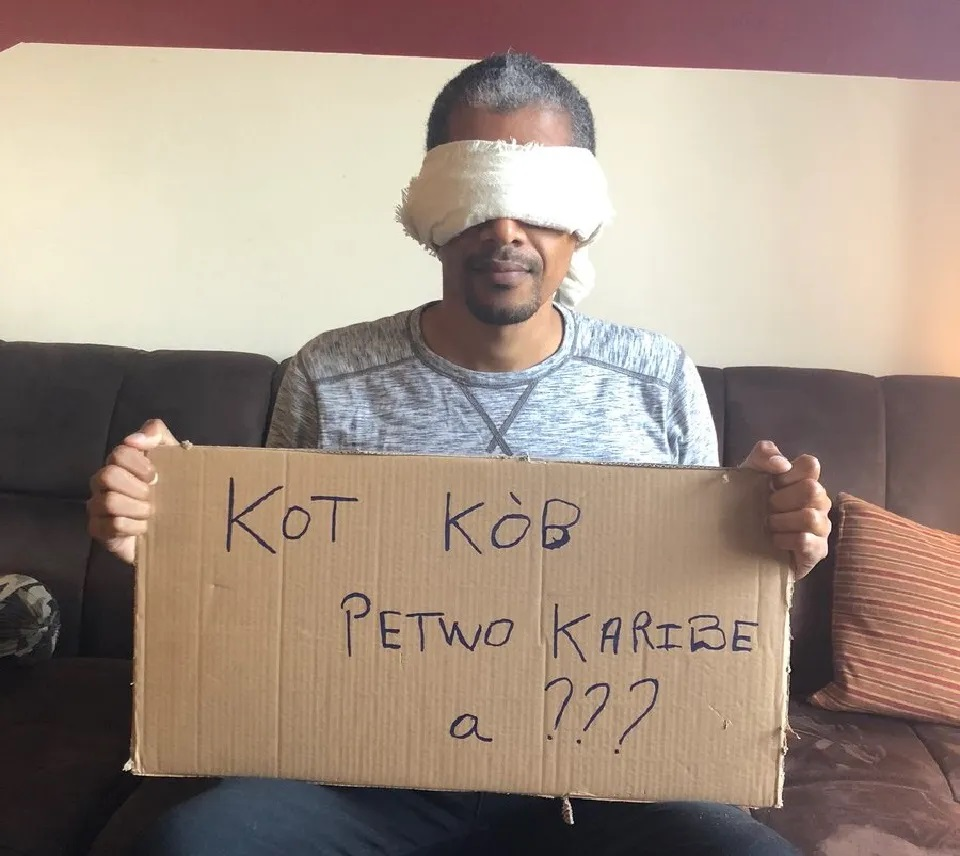
\includegraphics[height=5cm]{Pictures/PetroChallengerSlogan.jpg}
		\caption{Slogan du mouvement social ha\"itien Petro-Challengers\cite{PetroChallenger}}
		\label{Petrochallengers}
	\end{minipage}
	\hspace{10pt}
	\begin{minipage}{0.45\textwidth}
		\centering
		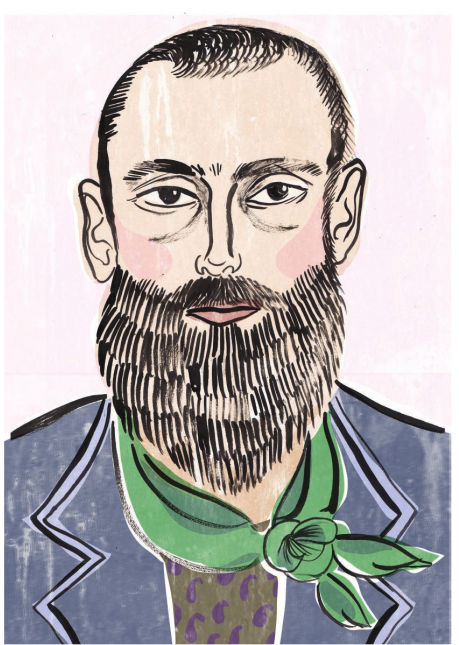
\includegraphics[height=5cm]{Pictures/IllustrationCommeArt.png}
		\caption{Image d'une illustration artistique\cite{ArtIllustre}}
		\label{IllustrationArt}
	\end{minipage}
\end{figure}

\subsubsection{Aide \`a la compr\'ehension}
Il s'agit l\`a de l'une des utilisations les plus r\'epandues des illustrations. Dans les livres, les articles, les sites internet et autres, les explications textuelles sont souvent accompagn\'ees d'illustrations graphiques pour offrir une expression plus claire des explications d\'ej\`a donn\'ees sous forme de texte (Voir Figure~\ref{CiscoReseau}).

\subsubsection{Art}
Les illustrations sont aussi utilis\'ees dans le domaine des arts, telle une fa\c{c}on cr\'eative, esth\'etique d'exprimer des id\'ees.(Voir figure~\ref{IllustrationArt}).


\section{Projets Similaires}
	Que ce soit pour Ha\"iti ou ailleurs, nous n'avons pas trouv\'e de projet ayant exactement le m\^eme objectif que le n\^otre: cr\'eer un syst\`eme d'information pour distribuer des illustrations afin de communiquer des informations sur les risques dans une r\'egion donn\'ee. Cependant, nous avons trouv\'e des projets qui abordent des aspects similaires. Pour ce document, nous nous proposons d'\'etudier trois groupes de projets suivant qu'ils consistent \`a cr\'eer un syst\`eme d'information pour pouvoir distribuer des documents via Internet, exploiter des illustrations dans un sens g\'en\'eral ou s'en servir pour enseigner.


	\subsection{Groupe 1 - Librairies en ligne}
		Une librairie en ligne est un site Internet qui fournit l'acc\`es \`a une collection de livres, articles, magazine, fichiers audio, images ou tout autre type de document accessible en ligne. Ces librairies peuvent offrir diff\'erents types de services notamment Le t\'el\'echargement, la lecture en ligne (streaming) ou le pr\^et (acc\`es pour une p\'eriode limit\'ee). Il existe beaucoup de librairie en ligne: Open Library, Europeana, Digital Public Library of America, The Online Books Page, Manybooks pour ne citer que quelques-unes. Elles se distinguent, entre autres, par la source des contenus propos\'es, leur public cible, les types de contenu propos\'e, les sujets couverts, le co\^ut d'acc\`es aux contenus ou leur politique d'utilisation et de redistribution des contenus. \`A titre d'exemple, nous pr\'esentons les d\'etails du projet Open Library.

		\subsubsection{Open Library}
			Open Library est un projet de Internet Archive\cite{InternetArchive} visant \`a rendre tous les livres accessibles \`a tous\cite{OpenLibVision}. C'est une librairie en ligne open source.\\

			\begin{itemize}
				\item[-] \textbf{Source des contenus}\\
				Les livres sur Open Library proviennent de sources divers, notamment, de partenariats, d'achats et de dons.\\

				\item[-] \textbf{Outils et technologies de d\'eploiement}\\
				Open library utilise Python comme langage de programmation, avec web.py comme framework ainsi qu'Infogami et Solr pour impl\'ementer certains services cot\'e serveur. Pour la base de donn\'ees, elle utilise PostgreSQL comme syst\`eme de gestion de base de donn\'ees et Memcached pour la gestion du cach. Cot\'e client, Open Library utilise Node.js pour la conception de l'interface web, Nginx pour g\'erer les requ\^etes des clients.\\

				\item[-] \textbf{Services offert}s\\
				Sur Open Library, vous pouvez lire un livre en ligne, l'\'ecouter, ou l'emprunter pour y acc\'eder hors ligne pendant une dur\'ee limit\'ee.\\

				\item[-] \textbf{Co\^uts et conditions d'acc\`es aux contenus}\\
				L'acc\`es aux livres est enti\`erement gratuit. Pour lire, \'ecouter, ou emprunter un livre, vous devez vous authentifier soit en cr\'eant un compte d'utilisateur ou en utilisant un compte Google.
			\end{itemize}





		\subsection{Groupe 2 - Projet de distribution d'illustrations}
			Une illustration \'etant avant tout un document, il est possible de trouver des illustrations dans toutes les librairies. De plus, il existe plusieurs sites web d\'edi\'es exclusivement \`a la distribution d'illustrations. Dont les suivants.\\

			\begin{itemize}
				\item[-] \textbf{Freepik}\\
					Freepik est une plateforme fond\'ee en 2010 par Alejandro Blanes, Pablo Blanes and Joaqu\'in Cuenca. Elle offre des illustrations de haute qualit\'e et propose une large gamme de ressources telles que des vid\'eos, des vecteurs, des photos, des maquettes, etc. Certaines de ces illustrations repr\'esentent des concepts li\'es \`a la gestion des risques comme \textbf{les s\'e\"isme, les temp\`ete, les catastrophes naturelles, etc} (Voir Figure~\ref{TempeteFromFreepik} et Figure~\ref{CatastropheNaturelleFromFreepik}). Freepik offre un acc\`es gratuit ainsi q'un acc\`es premium.\\

					\begin{figure}[ht]
						\vspace{10pt}
						\centering
						\begin{minipage}{0.45\textwidth}
							\centering
							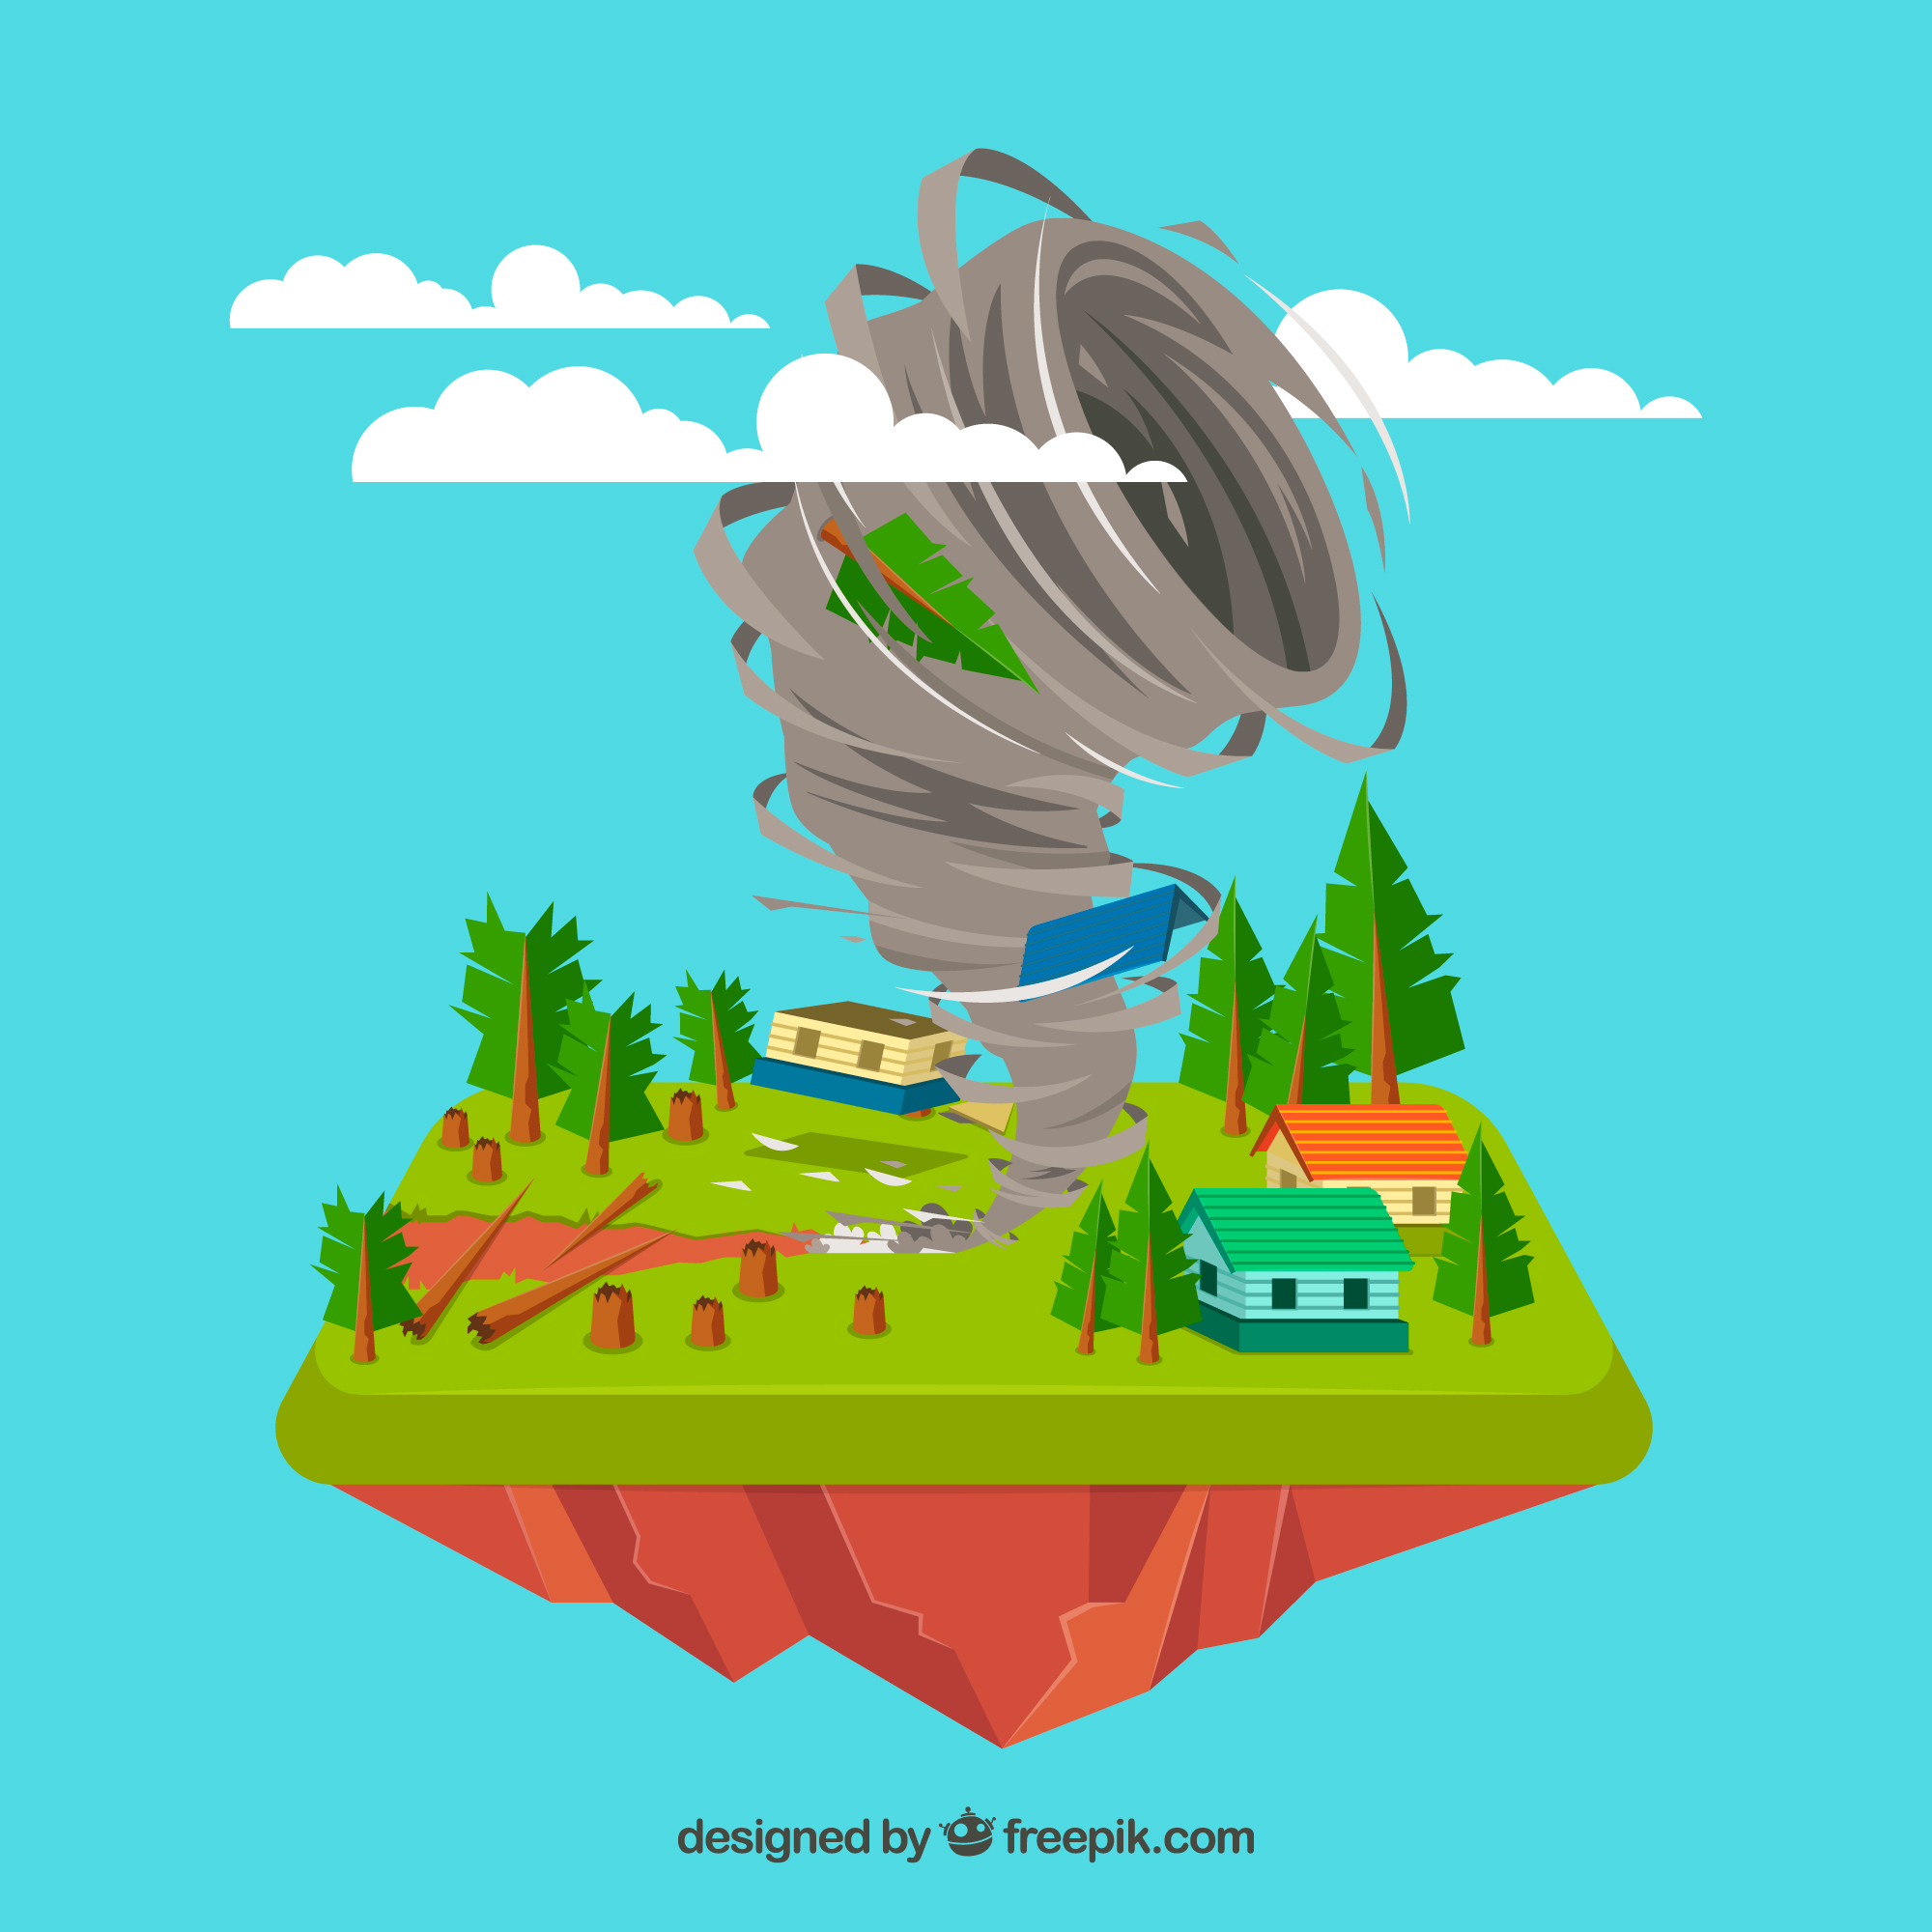
\includegraphics[width=5cm]{Pictures/CatastropheNaturelleFreepik.jpg}
							\caption{Illustration d'une catastrophe naturelle par \href{https://www.freepik.com/}{Freepik}}
							\label{CatastropheNaturelleFromFreepik}
						\end{minipage}
						\hspace{10pt}
						\begin{minipage}{0.45\textwidth}
							\centering
							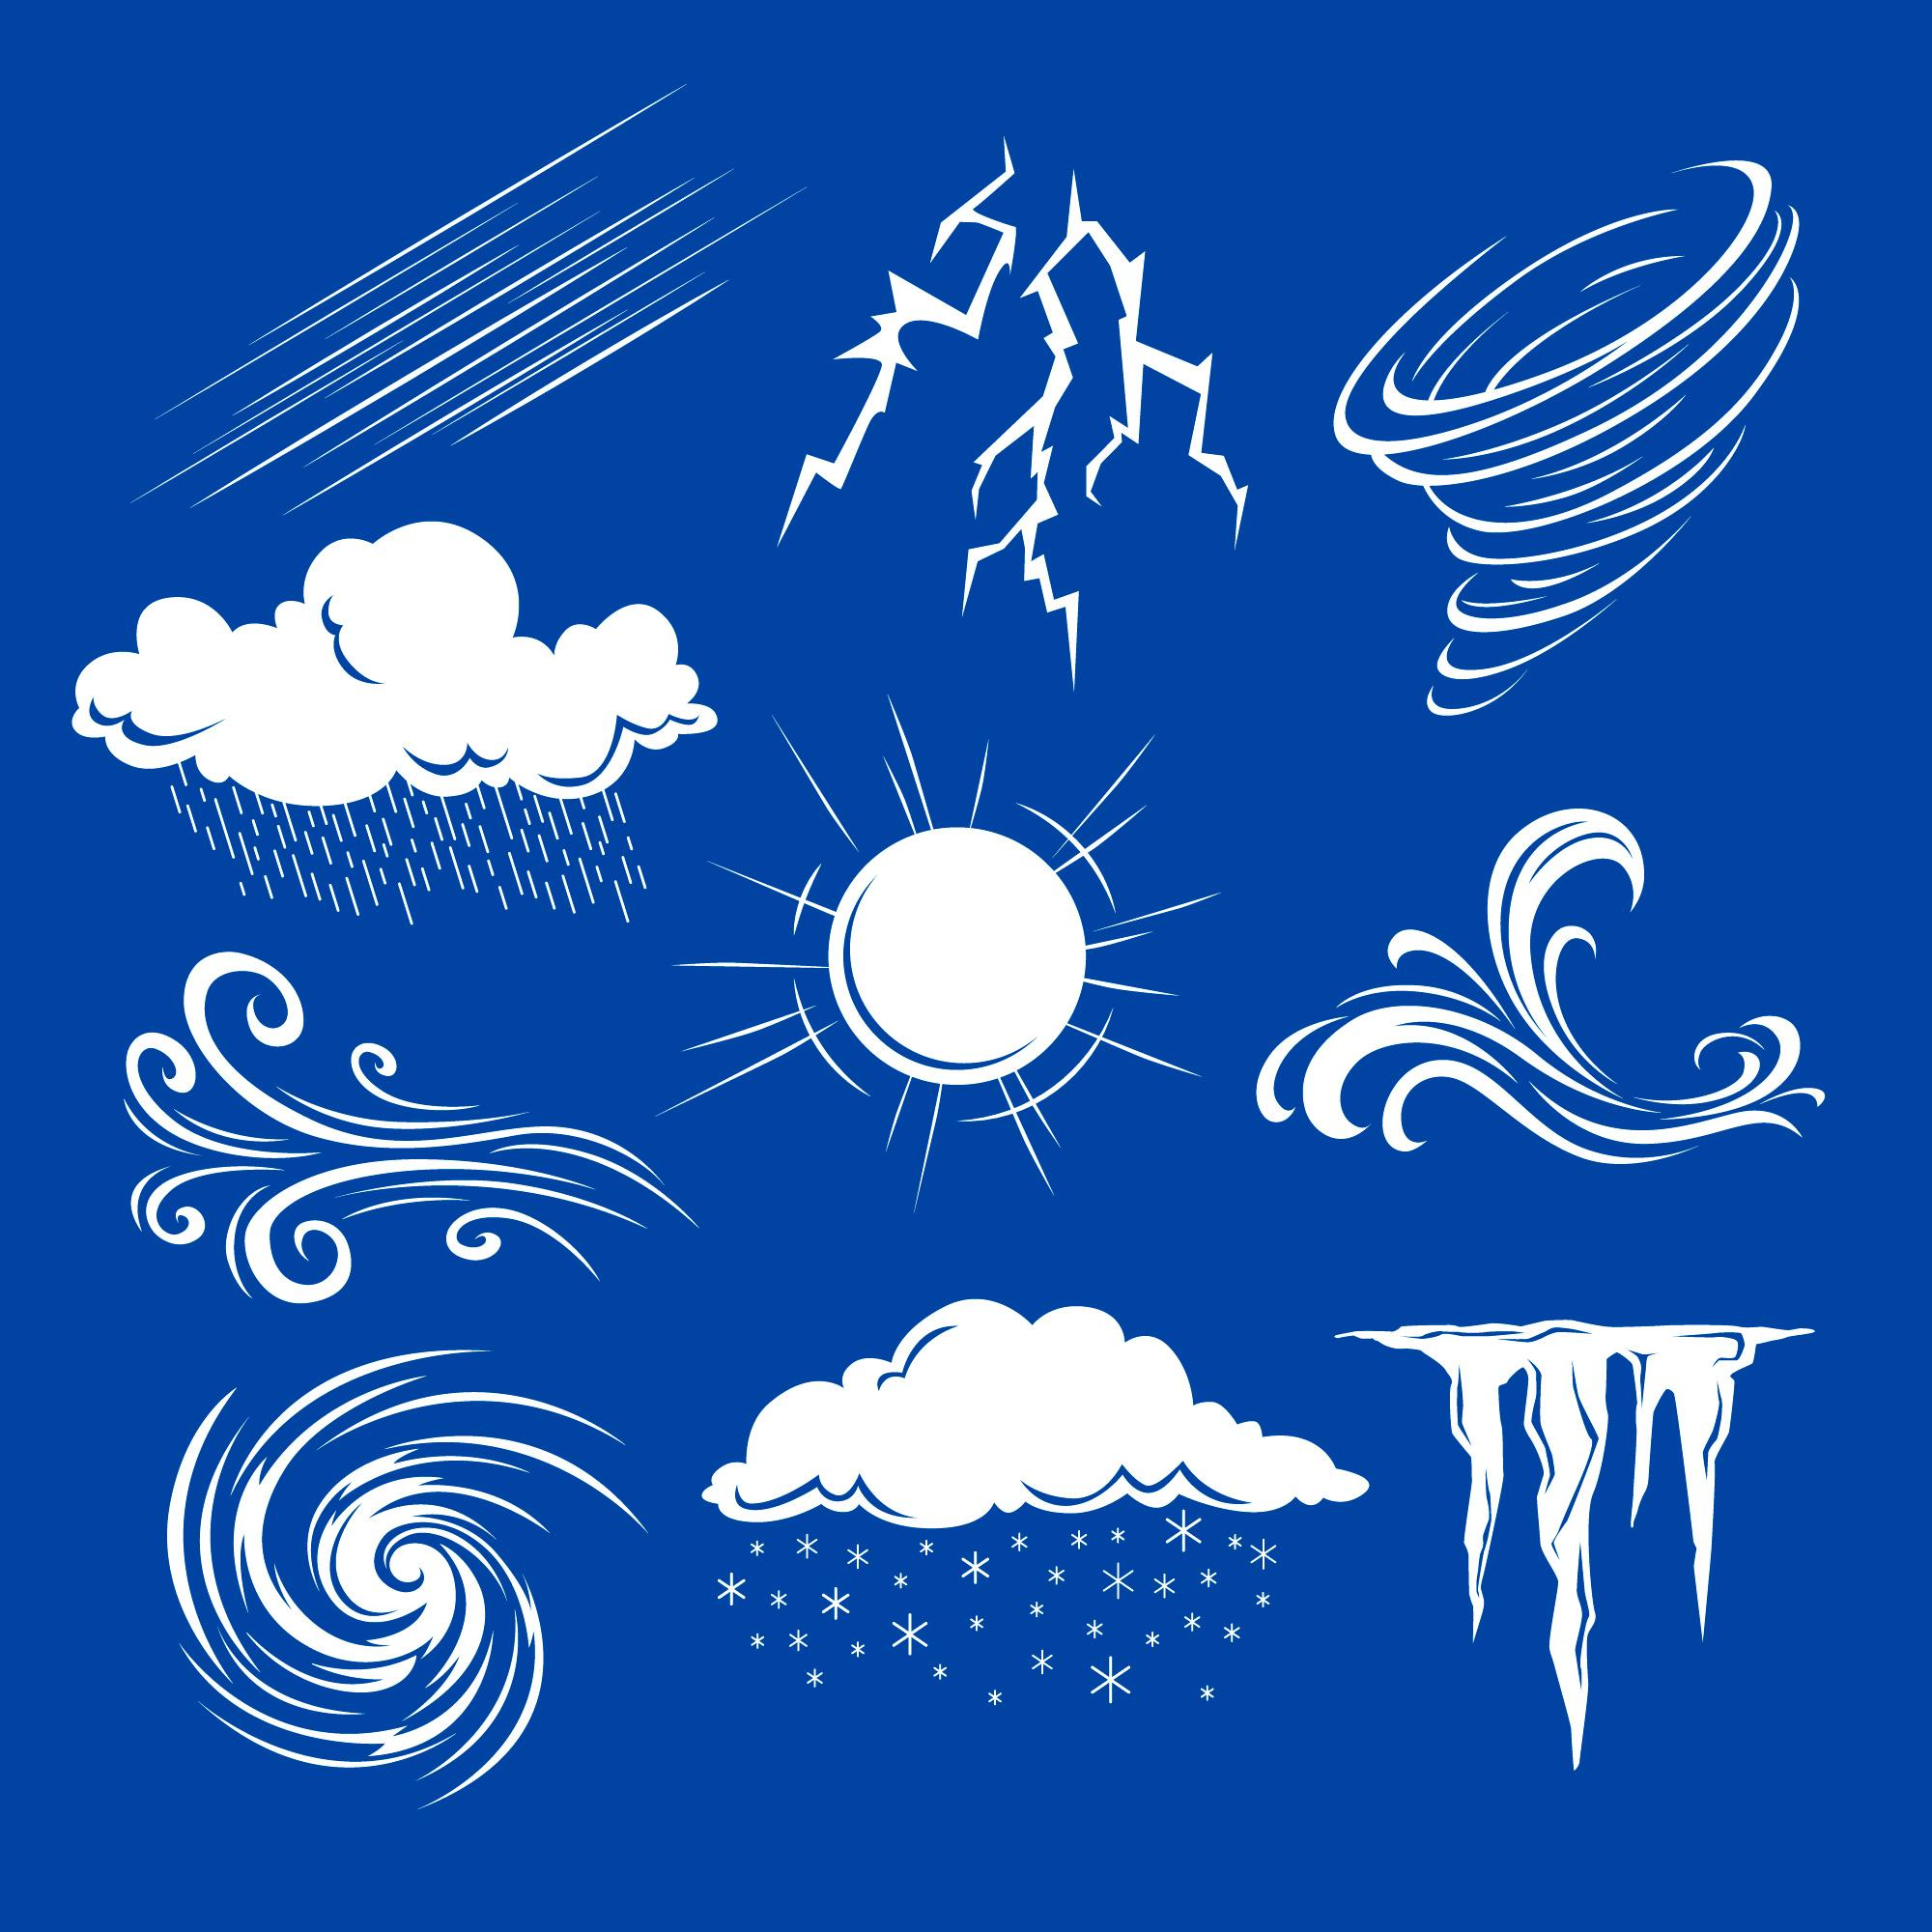
\includegraphics[width=5cm]{Pictures/TempeteFreepik.jpg}
							\caption{Illustration d'une temp\^ete par \href{https://www.freepik.com/}{Freepik}}
							\label{TempeteFromFreepik}
						\end{minipage}
					\end{figure}

				\item[-] \textbf{Pixabay}\\
					Pixabay est une plateforme de distribution d'illustrations gratuites sous licence libre. Elle fournit plus de 4 millions de vid\'eos, fichiers audio, images et autres m\'edias. On y trouve certains contenus qui concerne des concepts li\'es au risque.\\

				\item[-] \textbf{Craftwork}\\
					Craftwork Studio vous permet de commander des illustrations personnalis\'ees. Vous pouvez discuter avec eux de votre projet et des graphiques sp\'ecifiques dont vous aurez besoin. Ils cr\'eeront des \'ebauches initiales que vous pourrez examiner et commenter. Une fois le design affin\'e et parfait, vous recevrez votre design personnalis\'e.\\


				\item[-] \textbf{DesignCrowd}\\
					Sur DesignCrowd, vous pouvez lancer votre projet en leur indiquant ce dont vous avez besoin. Vous recevrez des propositions d'illustrations uniques du monde entier en quelques heures. Vous pouvez ensuite s\'electionner et approuver votre design pr\'ef\'er\'e et t\'el\'echarger les fichiers.


			\end{itemize}


		\paragraph{} De tous les projets que nous avons trouv\'e, le projet avec les objectif les plus proches du n\^otre en ce qui concerne les illustrations est \textbf{Kurzgesagt}.

\subsubsection{Kurzgesagt}
	Kurzgesagt est un studio d'animation allemand qui  vise \`a suciter la curiosit\'e de ses spectateurs et \`a encourager une vision du monde optimiste, bas\'ee sur la science et humaniste. Ainsi il travaille, entre autres, \`a produire des vid\'eos illustr\'es (graphes, animations, contexte narrative, ...) dans le but de vulgariser des connaissances scientifiques autour de sujets tels que la biologie, la physique, la chimie, l'\'economie ou l'astronomie en produisant notamment des videos illustr\'ees qu'il publient sur leurs cha\^ines YouTube. Les illustrations sont utilis\'ees pour rendre le contenu informatif amusant, esth\'etique et accessible \`a autant de gens que possible ind\'ependamment de leur \^age ou de leur formation acad\'emique.

	\begin{figure}[ht]
		\vspace{10pt}
		\centering
		\begin{minipage}{0.45\textwidth}
			\centering
			
\includegraphics[width=5cm]{Pictures/LogoKurzgesagt.png}
			\caption{Logo de \href{https://www.kurzgesagt.org/}{Kurzgesagt}}
			\label{LogoKurzgesagt}
		\end{minipage}
		\hspace{10pt}
		\begin{minipage}{0.45\textwidth}
			\centering
			
\includegraphics[width=7cm]{Pictures/AnimauxConnus.png}
			\caption{Image extraite de la vid\'eo \href{https://www.kurzgesagt.org/}{\textbf{\`A quoi ressemblaient VRAIMENT les dinosaures ?}} de Kurzgezagt.}
			\label{FigDino}
		\end{minipage}
	\end{figure}



\subsection{Groupe 3 - Utilisation des illustrations comme vecteur de communication}
Que ce soit sur les librairies qui distribuent des documents d'une fa\c{c}on g\'en\'erale ou parmi les projets qui se focalisent sur la distribution d'illustrations, nous trouvons des documents dans lesquels des illustrations sont utilis\'ees comme vecteur de communication. Dans cette cat\'egorie on retrouve les bandes d\'essin\'ees, les mangas comme moyen de communication, les livres pour enfant et bien d'autres ouvrages. La figure~\ref{FigDino} en est un exemple. Cette illustration repr\'esente nos connaissances sur les animaux tout en mettant l'emphase sur le fait le fait que certains nous sont encore inconnus.

\subsubsection{Alain Possible et le monde possible \cite{AlainPossible}}
Alain Possible et le Monde Possible est une s\'erie de bandes dessin\'ees publi\'ee par les Nations Unies dans le cadre d'une initiative soutenant les objectifs de d\'eveloppement durable en Ha\"iti. Le projet vise \`a sensibiliser les acteurs de la population locale aux objectifs de d\'eveloppement durable. Dans cette bande d\'essin\'ee, les illustrations sont utilis\'ees pour communiquer avec la population locale sur la signification du concept de d\'eveloppement durable, son importance, et les \'eventuels d\'eg\^ats que pourraient causer l'absence de sa prise en compte dans les projets \'etatiques (Voir Figure~\ref{TheTimeMachin}).




\begin{figure}[ht]
	\vspace{10pt}
	\centering
	\begin{minipage}{0.45\textwidth}
		\centering
		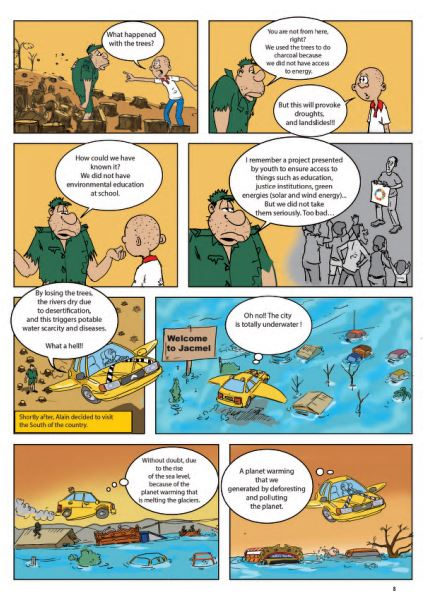
\includegraphics[width=5cm]{Pictures/AlainPossibleTheTimeMachine.jpg}
		\caption{Alain possible et le monde possible - La machine du temps / Page 8\cite{AlainPossible}}
		\label{TheTimeMachin}
	\end{minipage}
	\hspace{10pt}
	\begin{minipage}{0.45\textwidth}
		\centering
		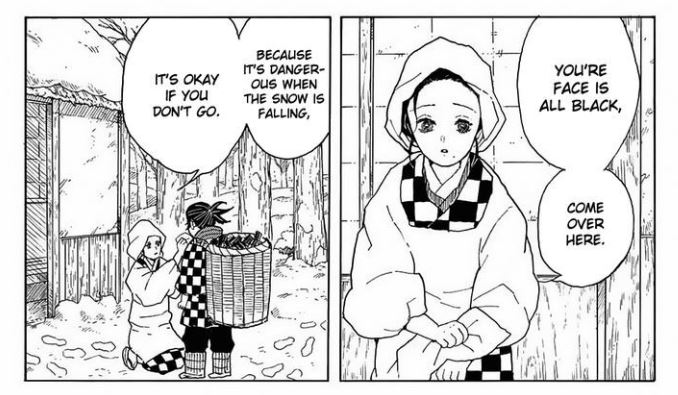
\includegraphics[height=5cm]{Pictures/DeKimetsuNoYaiba.jpg}
		\caption{Extrait de Kimetsu no yaiba}
		\label{DemonSlayer}
	\end{minipage}
\end{figure}

\subsubsection{Kimetsu no yaiba}
Kimetsu no yaiba est une s\'erie de manga \'ecrite et d\'essin\'ee par Koyoharu Got\=oge tr\`es connue depuis le d\'ebut des ann\'ees 2020. Il s'agit d'un ouvrage dans lequel illustrations sont utilis\'ees comme moyen de communiquer. (Voir Figure~\ref{DemonSlayer})

\subsubsection{Le petit prince\cite{LePetitPrince}}
Le petit prince est un livre d'Antoine De Saint Exup\'ery dans lequel l'auteur raconte l'histoire d'un enfant pour illustrer ses valeurs et les communiquer aux lecteurs.


\subsubsection{Kurzgesagt}
Kurzgesagt utilise aussi des illustrations comme vecteur de communication. Parfois, pour exprimer une id\'ee, au lieu de produire une expos\'ee explicative, il int\`egre leur id\'ee dans une histoire ou un cas concret. De plus dans toutes leurs vid\'eos, la partie visuelle est une s\'erie de dessins anim\'es qui illustre ce qui est dit. Prenons, par exemple, la vid\'eo \href{https://www.kurzgesagt.org/}{Et si nous atomisions une ville ?}%\cite{BombeAtomique}
. Au lieu d'une approche direct, c'est-\`a-dire, d\'efinir directement ce qu'est une bombe atomique, d\'ecrire son fonctionnement, pr\'esenter une liste des diff\'erentes r\'eactions qui font suite \`a son explosion et leur potentielles cons\'equences sur le milieu. La vid\'eo \'evalue ce qui passe alors qu'une bombe atomique vient d'exploser dans une ville. En pr\'esentant des observations bri\`evement expliqu\'ees sur ce qui s'est pass\'e dans la ville fictive, toutes les informations cit\'ees ci-dessus sont transmises. En plus, au lieu de devoir ajouter une section pour expliquer que les gens ayant surv\'ecu seront paniqu\'es, cette information est juste illustr\'ee \`a travers l'animation (Pendant quelques secondes, l'animation est celui du point de vue d'une personne qui sort des d\'ecombres, boulvers\'ee, perdue, paniqu\'ee, ...).\\
Ce projet, en soi, est un bon exemple de l'utilisation d'illustrations \`a une telle fin. Elle permet aussi d'observer l'efficacit\'e de cette m\'ethode de communication. En effet, en tr\`es peu de temps, la cha\^ine anglophone a atteint 20 Millions d'abonn\'es(es). En plus les commentaires laiss\'ees sous les vid\'eos laissent croire que les sont gens sont tr\`es satisfaits par la forme de la pr\'esentation.



